\documentclass[11pt]{article}
\usepackage[margin=1in]{geometry}
\usepackage{parskip}
\usepackage{hyperref}
\usepackage{lmodern}
\usepackage[T1]{fontenc}
\usepackage[utf8]{inputenc}
\usepackage{setspace}
\usepackage{enumitem}
\usepackage{pdfpages}

\hypersetup{colorlinks=true,linkcolor=black,urlcolor=blue}

\begin{document}

\noindent\textbf{\Large Amirehsan Davoodi}

\vspace{6pt}

\noindent\begin{tabular*}{\textwidth}{@{\extracolsep{\fill}} l r}
    \href{mailto:amirehsan.davoodi@gmail.com}{amirehsan.davoodi@gmail.com} & Tehran, Iran \\
    LinkedIn: \href{https://www.linkedin.com/in/amirehsan-davoodi}{linkedin.com/in/amirehsan-davoodi} & (+98)~915\,612\,6388 \\
\end{tabular*}

\vspace{6pt}

\noindent\begin{flushright}
    \today
\end{flushright}

\vspace{0.5cm}

\textbf{To:} Prof. Dr. Christian Ledig\\
Chair of Explainable Machine Learning\\
Otto-Friedrich-Universit\"at Bamberg\\
An der Weberei 5, D-96047 Bamberg\\
\href{mailto:christian.ledig@uni-bamberg.de}{christian.ledig@uni-bamberg.de}

\vspace{0.5cm}

\section*{Motivation Letter}
Dear Prof. Ledig,

I am writing to apply for the Doctoral Student / PostDoc position at the Chair of Explainable Machine Learning. My research focuses on reliable, data-efficient, and interpretable machine learning for time-series and imaging data, with an emphasis on agentic AI systems and explainable representations. This opportunity aligns strongly with my background and interests in robust deep learning, knowledge representation, and medical AI.

I am currently a PhD candidate in AI at Amirkabir University of Technology (AGML Center) and hold an MSc in AI from USI (Universit\`a della Svizzera italiana), Lugano. I combine research and engineering experience (Python, PyTorch, FastAPI, Docker) with a publication track that includes graph learning for fMRI-based autism diagnosis (ASD-GraphNet; Computers in Biology and Medicine, 2025; \href{https://doi.org/10.1016/j.compbiomed.2025.110723}{doi:10.1016/j.compbiomed.2025.110723}) and an under-review paper on an agentic AI framework for knowledge graph construction (HIDE-KG). During my Master’s, I co-founded the startup UbiHealth (covered by USI News) and completed the Innosuisse Entrepreneurship Training in Ticino.

Methodologically, I work on: (i) dual-learning validation loops to improve reliability (text-based reconstruction and re-parsing for knowledge structures), (ii) representation learning for graphs and time-series (including self-/weakly-supervised setups), and (iii) XAI with perturbation-based and counterfactual analyses. These directions map well to your group’s topics: robustness/generalization, data efficiency, outlier detection, and interpretable evaluation in healthcare and medical imaging contexts.

I would be excited to contribute to your lab’s research and teaching, collaborate with the Bamberg Center for AI, and publish at top venues (CVPR/ICCV/ECCV/AAAI/MICCAI). I would welcome the opportunity to discuss how my background can support your group’s goals.

Sincerely,\\[6pt]
\textbf{Amirehsan Davoodi}

\vspace{0.6cm}

\section*{Curriculum Vitae (Concise)}
\textbf{Education}
\begin{itemize}[leftmargin=*]
    \item PhD Candidate, Artificial Intelligence, Amirkabir University of Technology (AGML Center), Tehran
    \item MSc, Artificial Intelligence, Universit\`a della Svizzera italiana (USI), Lugano
\end{itemize}

\textbf{Selected Research}
\begin{itemize}[leftmargin=*]
    \item HIDE-KG (under review): Hierarchical Dual-learning Entity-clustered Knowledge Graph Construction Using Pre-trained LLMs (agentic AI + dual validation for reliability)
    \item ASD-GraphNet (2025): fMRI-based autism diagnosis via graph learning (Computers in Biology and Medicine; \href{https://doi.org/10.1016/j.compbiomed.2025.110723}{doi:10.1016/j.compbiomed.2025.110723})
    \item Master’s thesis: Goal-directed graph generation for anomaly detection on time series (ECG arrhythmia)
\end{itemize}

\textbf{Industry/Applied Experience}
\begin{itemize}[leftmargin=*]
    \item Software/ML Engineer (FastAPI, PyTorch, LangChain, Docker, PostgreSQL/MongoDB)
    \item Tali AI (Toronto): AI assistant and data platform contributions
    \item Co-founder, UbiHealth (remote patient monitoring; \href{https://www.usi.ch/en/feeds/8176}{USI News}); Innosuisse Entrepreneurship Training (Ticino)
\end{itemize}

\textbf{Skills}
\begin{itemize}[leftmargin=*]
    \item ML/DL: PyTorch, scikit-learn, XGBoost; self-/weakly-supervised learning; outlier detection
    \item XAI: perturbation-based and feature attribution methods; uncertainty estimation
    \item Systems: Python, FastAPI, Docker; experiment tracking; reproducible pipelines
\end{itemize}

\vspace{0.6cm}

\section*{Research Proposal (Summary)}
\textbf{Title:} Dual-Learning and Perturbation-based Explainability for Time-series Graph Representations

\textbf{Motivation:} Reliability and interpretability remain key bottlenecks in deploying neural networks for healthcare and related domains. Many signals are temporal and multi-source (wearables, EHR, imaging-derived time-series), where structure emerges across channels and time. Knowledge graphs (KGs) and graph neural networks (GNNs) offer a natural abstraction for capturing dependencies, but require robust validation and explainability.

\textbf{Aim:} Develop a dual-learning validation framework and perturbation-based explainability for knowledge graphs derived from time-series data (uni- and multivariate). The approach targets robust generalization, outlier detection, and quantifiable uncertainty while maintaining clinically meaningful interpretability.

\textbf{Objectives:}
\begin{enumerate}[leftmargin=*]
    \item \textit{Time-series to Graph Construction:} Design pipelines that map time-series to graphs via similarity, causality, or learned relational structure; support dynamic/temporal graphs.
    \item \textit{Dual-learning Validation:} Extend dual reconstruction (graph-to-text and text-to-graph; or graph-to-signal and signal-to-graph) to assess fidelity, flag hallucinations/spurious edges, and calibrate uncertainty.
    \item \textit{Perturbation-based XAI for Graphs:} Introduce a principled perturbation scheme on graph-structured time-series (node/edge/channel/time masking, controlled noise, counterfactual rewiring) to quantify feature importance and stability.
    \item \textit{Data Efficiency \& Robustness:} Employ self-/weakly-supervised objectives and outlier-aware training to improve performance under limited labels and distribution shifts.
    \item \textit{Evaluation in Medical Settings:} Validate on benchmark datasets (ECG, PPG, EEG, fMRI-derived timeseries) with metrics covering accuracy, calibration, and explanation faithfulness.
\end{enumerate}

\textbf{Methods:}
\begin{itemize}[leftmargin=*]
    \item GNNs for temporal graphs; contrastive/self-supervised pretraining; uncertainty via ensembles or evidential methods
    \item Dual-learning loops for structural fidelity; text/signal reconstruction checks; graph edit distance and information-theoretic criteria
    \item Perturbation generators respecting temporal and physiological constraints; attribution stability and counterfactual validity tests
\end{itemize}

\textbf{Outcomes:} (i) Reliable graph construction from time-series; (ii) robust models with calibrated uncertainty; (iii) interpretable, perturbation-grounded explanations; (iv) open-source code and reproducible benchmarks; (v) publications targeting CVPR/ICCV/ECCV/AAAI/MICCAI.

\clearpage
\section*{Appendix: Transcripts}
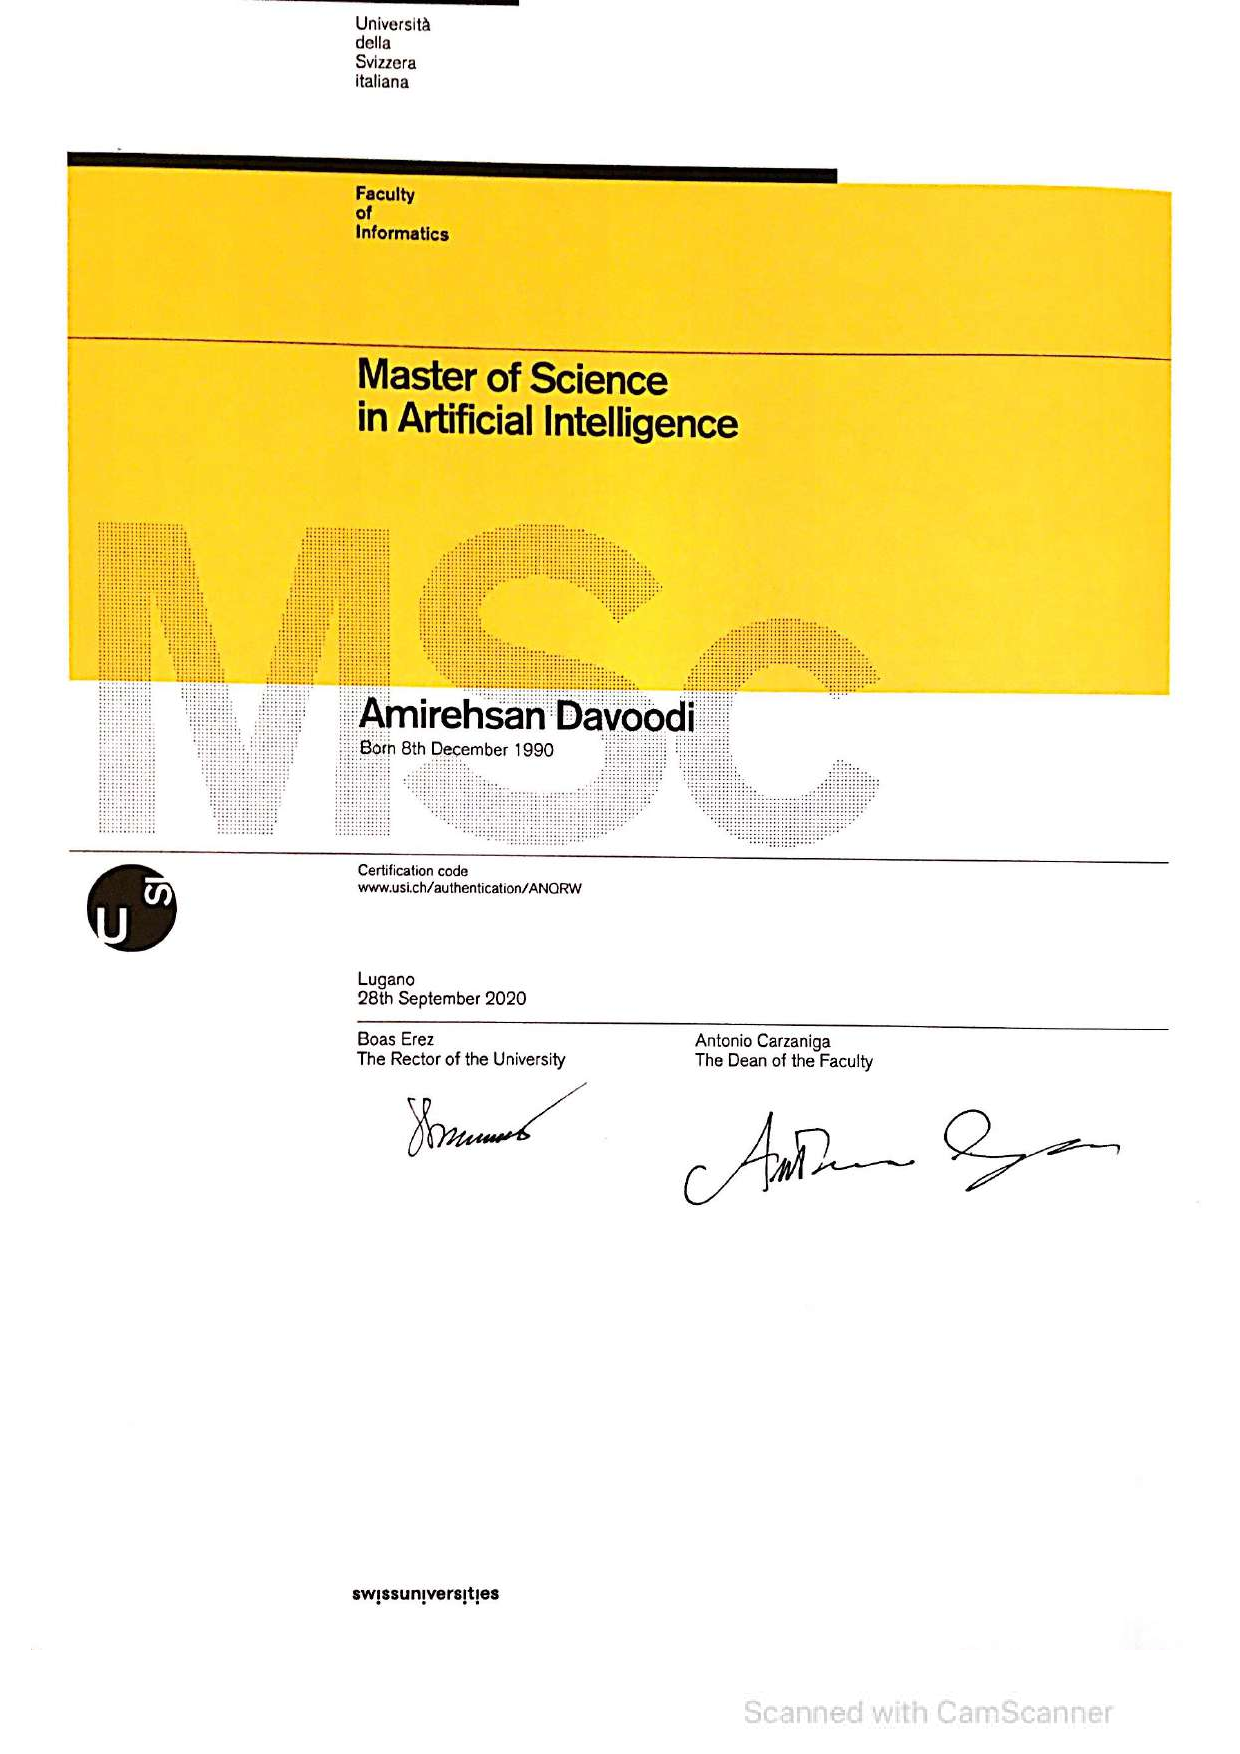
\includepdf[pages=-]{/home/ehsan/Documents/private/Research Positions applications/MasterDiploma_Supplement_compressed.pdf}

\end{document}


